% !TeX program = xelatex
% !TeX encoding = UTF-8
% !TeX TXS-program:compile = txs:///xelatex | txs:///xelatex
\documentclass[aspectratio=169, table, 12pt]{beamer}

% Preamble bersama seluruh slide mata kuliah ini.
% Dipanggil dari slides/sessionXX/sessionXX.tex tepat sesudah baris
% \documentclass[aspectratio=169, table, 12pt]{beamer}
% Paket tambahan yang hanya dibutuhkan satu sesi ditulis di berkas sesi itu.

\usepackage{colortbl}
\usepackage{xcolor}
\usepackage{listings}
\usepackage{tabularx}
\usepackage{booktabs}
\usepackage{tikz}
\usepackage{pgfplots}
\usepackage{fontspec}
\usepackage[english,bahasai]{babel}
\pgfplotsset{compat=1.18}
\usetikzlibrary{arrows.meta, positioning, calc, fit, shapes.geometric,
  shapes.multipart, backgrounds, matrix, chains, trees}

\makeatletter
\def\input@path{{../theme/}}
\makeatother
\graphicspath{{../theme/}{../../figures/}}
% Stub symlink Windows memakai tema cadangan sampai aset institusi tersedia.
\IfFileExists{../theme/beamerthemePradita.sty}{%
  \usetheme{Pradita}
}{%
  \usetheme{Madrid}
  \setmainfont{TeX Gyre Heros}
  \setsansfont{TeX Gyre Heros}
  \setbeamertemplate{navigation symbols}{}
}

\definecolor{praditagreen}{RGB}{37, 113, 71}
\setbeamercolor{structure}{fg=praditagreen}
\setbeamercolor{palette primary}{bg=praditagreen,fg=white}
\setbeamercolor{palette secondary}{bg=praditagreen!80!black,fg=white}
\setbeamercolor{palette tertiary}{bg=praditagreen!60!black,fg=white}
\setbeamerfont{frametitle}{size=\large}
\setbeamertemplate{caption}[numbered]

% Ukuran header mengikuti teks agar judul panjang tidak menabrak logo.
\setbeamercolor{frametitle}{bg=white,fg=black}
\setbeamertemplate{frametitle}{%
  \begin{beamercolorbox}[wd=\paperwidth,sep=0.2cm]{frametitle}
    \begin{minipage}[c]{0.77\paperwidth}
      \raggedright\fontsize{16}{18}\selectfont\bfseries\insertframetitle
      \ifx\insertframesubtitle\empty\else
        \par\small\mdseries\insertframesubtitle
      \fi
    \end{minipage}\hfill
    \begin{minipage}[c]{0.15\paperwidth}
      \IfFileExists{../theme/classFiles/logo_universitas.png}{%
        
\includegraphics[width=\linewidth]{../theme/classFiles/logo_universitas.png}%
      }{}
    \end{minipage}
  \end{beamercolorbox}
}
\setbeamertemplate{footline}{%
  \ifnum\value{framenumber}>1
    \begin{beamercolorbox}[wd=\paperwidth,ht=0.35cm,dp=0.15cm,
      leftskip=0.3cm,rightskip=0.3cm]{palette primary}
      \footnotesize\bfseries\insertframenumber/\inserttotalframenumber
      \hfill IT40513
    \end{beamercolorbox}
  \fi
}
\DeclareRobustCommand{\berkas}[1]{\path{#1}}

% Tema membuat garis tabel berwarna putih. Dikembalikan agar tabel terbaca.
\arrayrulecolor{black}
\setlength{\arrayrulewidth}{0.5pt}

\lstdefinelanguage{yaml}{
  basicstyle=\ttfamily\scriptsize,
  keywordstyle=\color{blue}\bfseries,
  commentstyle=\color{gray}\itshape,
  stringstyle=\color{red},
  showstringspaces=false,
  breaklines=true,
  frame=lines,
  numbers=none,
  backgroundcolor=\color{lightgray!10},
  tabsize=2,
  morecomment=[l]{\#}
}

\lstdefinelanguage{json}{
  basicstyle=\ttfamily\scriptsize,
  stringstyle=\color{red},
  commentstyle=\color{gray},
  breaklines=true,
  showstringspaces=false,
  tabsize=2,
  numbers=none,
  frame=lines,
  backgroundcolor=\color{lightgray!10},
  string=[s]{"}{"}
}

\lstdefinelanguage{bash}{
  keywords={},
  basicstyle=\ttfamily\scriptsize,
  ndkeywords={docker, kubectl, helm, curl, git, terraform},
  ndkeywordstyle=\color{purple}\bfseries,
  sensitive=true,
  commentstyle=\color{gray},
  numbers=none,
  breaklines=true,
  frame=lines,
  backgroundcolor=\color{lightgray!10},
  tabsize=2,
  comment=[l]{\#},
  showstringspaces=false
}

\lstdefinelanguage{http}{
  keywords={GET, POST, PUT, PATCH, DELETE, HEAD, OPTIONS, HTTP},
  basicstyle=\ttfamily\scriptsize,
  keywordstyle=\color{blue}\bfseries,
  sensitive=true,
  numbers=none,
  breaklines=true,
  frame=lines,
  backgroundcolor=\color{lightgray!10},
  tabsize=2,
  showstringspaces=false
}

\subtitle{IT40513 · Enterprise Architecture \& Digital Blueprint}
\author{\textbf{Alfa Yohannis}}


% Sampul membatasi judul di panel putih tema rujukan Pradita.
\setbeamertemplate{title page}{%
  \begin{tikzpicture}[remember picture,overlay]
    \node[anchor=north west,inner sep=0pt,text width=8.8cm]
      at ([xshift=1cm,yshift=-3.15cm]current page.north west) {%
        {\small\insertsubtitle\par}\vspace{0.25cm}
        \resizebox{8.8cm}{!}{\begin{minipage}{12cm}
          \raggedright\color{praditagreen}\bfseries\inserttitle
        \end{minipage}}
      };
    \node[anchor=south west,inner sep=0pt]
      at ([xshift=1cm,yshift=1.65cm]current page.south west)
      {\small\insertdate};
    \node[anchor=west,inner sep=0pt,text=white]
      at ([xshift=0.8cm,yshift=0.75cm]current page.south west)
      {\small\insertauthor};
  \end{tikzpicture}
}


% Batasi kedua dimensi gambar agar diagram bersama tetap berada pada slide.
\newsavebox{\eafigbox}
\newcommand{\eadiagram}[1]{%
  \sbox{\eafigbox}{\resizebox{0.94\textwidth}{!}{\input{#1}}}%
  \ifdim\dimexpr\ht\eafigbox+\dp\eafigbox\relax>0.64\textheight
    \resizebox{!}{0.64\textheight}{\usebox{\eafigbox}}%
  \else
    \usebox{\eafigbox}%
  \fi
}


\newcolumntype{Y}{>{\raggedright\arraybackslash}X}
\newcolumntype{L}[1]{>{\raggedright\arraybackslash}p{#1}}

% Font tema slide lebih lebar daripada font modul, sehingga kotak jaringan manfaat
% bersentuhan. Lebar kotak dan jarak mendatarnya dilonggarkan khusus di slide ini.
\makeatletter
\newcommand{\longgarkandiagram}[2]{%
  \tikzset{text width/.code={\def\tikz@text@width{#1}},
           every picture/.append style={x=#2}}}
\makeatother

\title{\Huge Business Case dan\\ \vspace{10pt} Portofolio Inisiatif}
\date{Pertemuan 13}

\begin{document}

\frame{\titlepage}

\begin{frame}
  \frametitle{Isi Pertemuan}
  \vspace{14pt}
  \begin{columns}[t]
    \column{0.5\textwidth}
    {\small\tableofcontents[sections={1-4}]}

    \column{0.5\textwidth}
    {\small\tableofcontents[sections={5-7}]}
  \end{columns}
\end{frame}

\begin{frame}{\hfill}
  \centering
  \Huge{\textbf{Proyek selesai tepat waktu,\\lalu apa hasilnya\\bagi organisasi?}}
\end{frame}

\section{Tujuan dan Konteks}

\begin{frame}{\hfill}
  \centering
  \Huge{\textbf{Tujuan dan Konteks}}
\end{frame}

\begin{frame}{{\Large Tujuan Pembelajaran}}
  \vspace{10pt}
  \begin{itemize}
    \item Menyusun \textit{business case} untuk inisiatif prioritas dengan manfaat, biaya, risiko, dan
          asumsi yang eksplisit.
    \item Memetakan manfaat ke perubahan bisnis dan pemungkinnya dengan \textit{benefits dependency
          network}.
    \item Memprioritaskan portofolio inisiatif dengan kriteria berbobot dan menjustifikasi hasilnya.
  \end{itemize}
\end{frame}

\begin{frame}{{\Large Masalah: Proyek Selesai, Hasil Tidak Diketahui}}
  \small
  \vspace{6pt}
  \begin{itemize}
    \item Laporan penutupan proyek Teknologi Informasi (TI) menyatakan tepat waktu dan sesuai anggaran.
    \item Setahun kemudian seorang komisaris menanyakan hasilnya, dan tidak ada yang dapat menjawab.
    \item Sejak awal tidak ada yang menetapkan hasil, penanggung jawab, dan cara mengukurnya.
    \item Bab 12 menjawab apa yang dikerjakan lebih dahulu.
    \item Bab ini menjawab dua hal: mengapa inisiatif layak didanai, dan mana yang didanai bila uang
          tidak cukup.
  \end{itemize}
\end{frame}

\begin{frame}{{\Large Diagram Konsep Bab 13}}
  \centering
  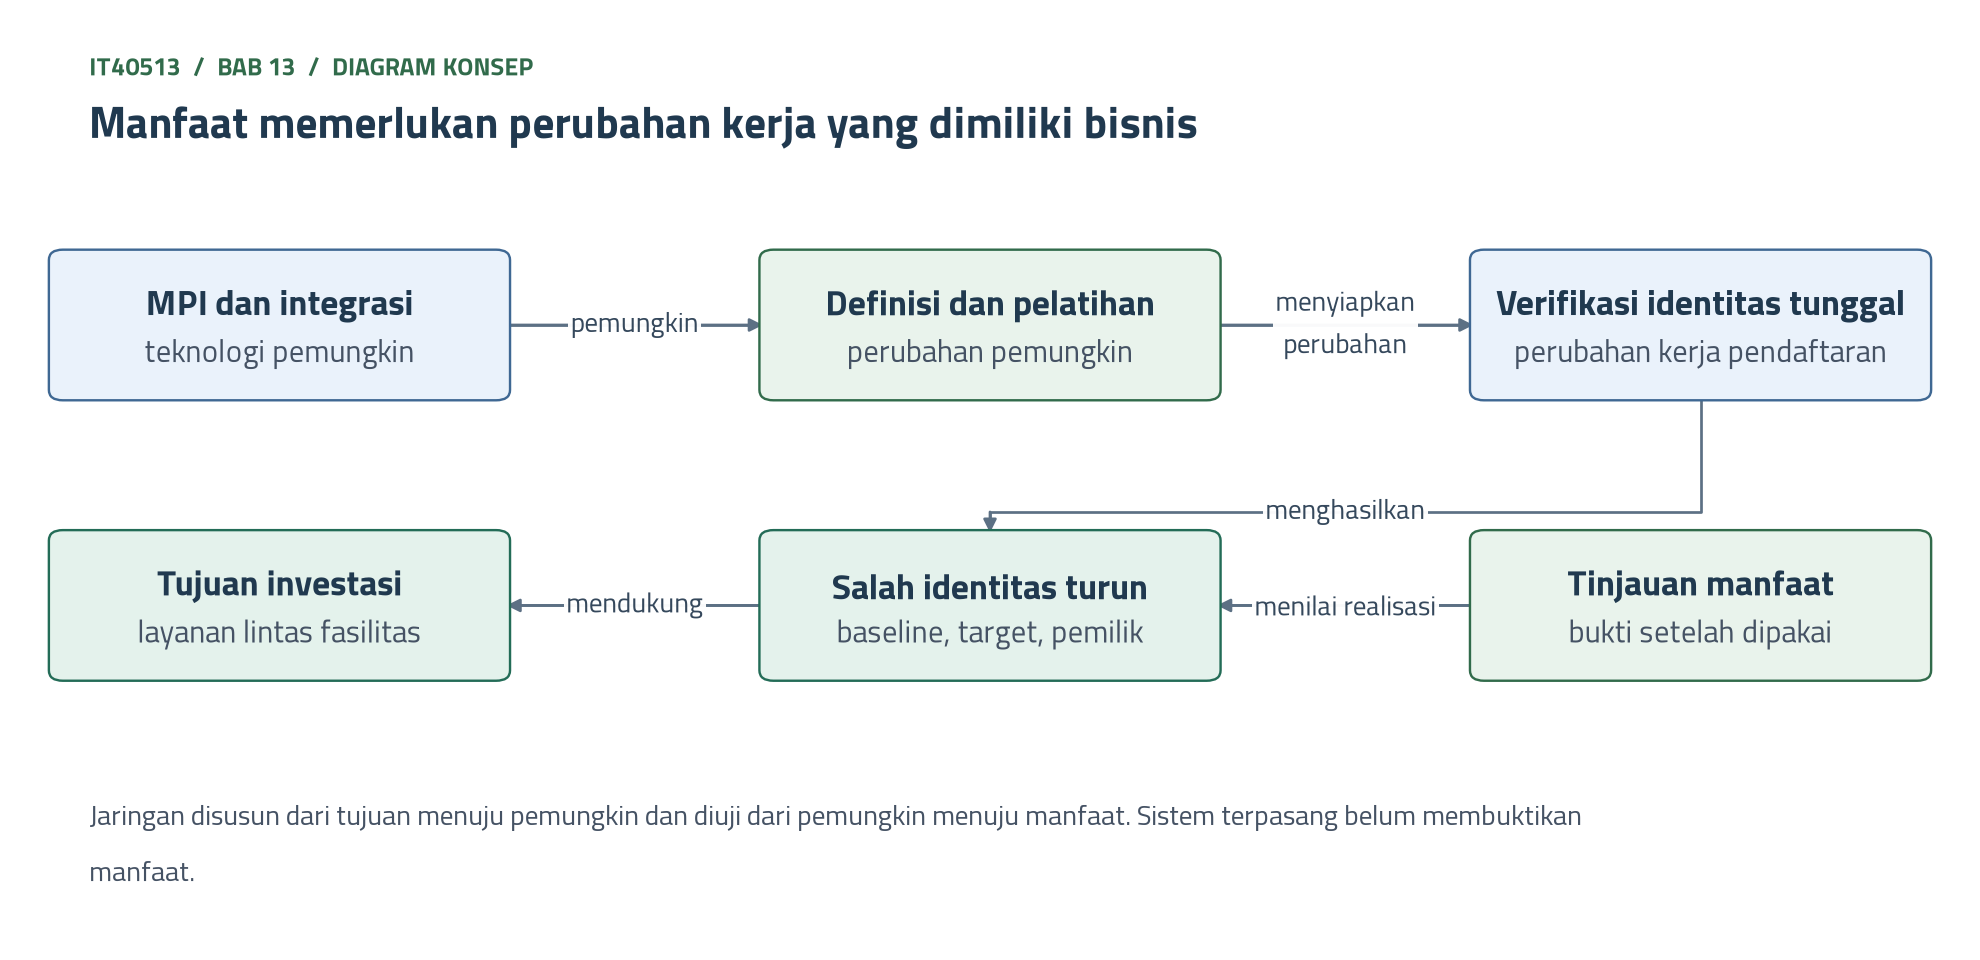
\includegraphics[width=0.96\textwidth,height=0.77\textheight,keepaspectratio]{../../figures/ch13-diagram-konsep.png}
  \label{fig:session13-ilustrasi-bab}
\end{frame}

\section{Manajemen Manfaat}

\begin{frame}{\hfill}
  \centering
  \Huge{\textbf{Manajemen Manfaat}}
\end{frame}

\begin{frame}{{\Large Teknologi Tidak Menghasilkan Manfaat}}
  \small
  \vspace{6pt}
  \begin{itemize}
    \item Manajemen manfaat (\textit{benefits management}) mengatur investasi TI agar manfaat benar-benar
          terwujud.
    \item Manfaat muncul ketika orang bekerja dengan cara baru yang dimungkinkan teknologi.
    \item Manfaat dinyatakan sebagai perubahan ukuran kinerja, bukan daftar kemampuan sistem.
    \item Pemilik manfaat (\textit{benefit owner}) menerima manfaat itu dan berwenang mengubah cara kerja
          unitnya.
  \end{itemize}
  \vspace{6pt}
  Analogi: \textit{treadmill} tanpa perubahan kebiasaan berakhir menjadi gantungan baju, padahal
  ``proyek pembelian''-nya selesai tepat waktu.
\end{frame}

\begin{frame}{{\Large Fitur, Manfaat, dan Perubahan Cara Kerja}}
  \footnotesize
  \begin{tabularx}{\textwidth}{YYY}
    \hline
    \textbf{Fitur yang dibeli} & \textbf{Manfaat yang diharapkan} &
      \textbf{Perubahan cara kerja yang dibutuhkan} \\
    \hline
    Pencarian pasien di MPI & Pendaftaran pasien lama turun dari 6 menjadi
      3 menit & Petugas mencari pasien lebih dahulu sebelum membuat rekam
      medis baru \\
    \hline
    Janji temu daring di Medikara+ & Antrean loket pagi berkurang & Dokter
      membuka kuota jadwal di aplikasi, bukan hanya di loket \\
    \hline
    \textit{Dashboard} laporan terpadu & Rapat bulanan tanpa rekonsiliasi angka
      & Unit berhenti menyusun \textit{spreadsheet} sendiri \\
    \hline
    Peninjauan hak akses otomatis & Temuan audit kontrol akses ditutup &
      Atasan meninjau hak akses bawahannya tiap triwulan \\
    \hline
  \end{tabularx}

  \vspace{6pt}
  \small MPI (\textit{Master Patient Index}) adalah indeks identitas pasien tunggal dari Bab 9.
\end{frame}

\begin{frame}{{\Large Siklus Manajemen Manfaat}}
  \small Perubahan cara kerja direncanakan, dianggarkan, dan dipantau seperti perangkat lunaknya.
  Tahap keempat menyambung ke tata kelola Bab 14.

  \centering
  \begin{figure}
    \resizebox{0.94\textwidth}{!}{\begin{tikzpicture}[
  font=\scriptsize,
  tahap/.style={draw, rounded corners, minimum height=1.25cm, text width=1.85cm,
                align=center, font=\scriptsize\bfseries},
  panah/.style={-{Stealth[length=2mm]}, thick}
]
  \node[tahap, fill=blue!8] (t1) at (0,0)
    {{\tiny\mdseries Tahap 1}\\Identifikasi dan susun manfaat};
  \node[tahap, fill=blue!8] (t2) at (2.45,0)
    {{\tiny\mdseries Tahap 2}\\Rencanakan realisasi manfaat};
  \node[tahap, fill=blue!8] (t3) at (4.9,0)
    {{\tiny\mdseries Tahap 3}\\Jalankan rencana manfaat};
  \node[tahap, fill=orange!12] (t4) at (7.35,0)
    {{\tiny\mdseries Tahap 4}\\Tinjau dan evaluasi hasil};
  \node[tahap, fill=green!10] (t5) at (9.8,0)
    {{\tiny\mdseries Tahap 5}\\Temukan manfaat lanjutan};

  \draw[panah] (t1) -- (t2);
  \draw[panah] (t2) -- (t3);
  \draw[panah] (t3) -- (t4);
  \draw[panah] (t4) -- (t5);
  \draw[panah] (t5.south) -- ++(0,-0.6) -| (t1.south);
  \node[font=\tiny, gray, fill=white, inner sep=1pt] at (4.9,-1.23)
    {investasi berikutnya memakai pelajaran dari siklus ini};

  \draw[gray, thick] ([yshift=0.15cm]t1.north west) -- ++(0,0.15)
    -- ([yshift=0.3cm]t2.north east) -- ++(0,-0.15);
  \node[font=\tiny, anchor=south] at ($(t1.north)!0.5!(t2.north)+(0,0.32)$)
    {\textit{business case} disusun di sini};
  \node[font=\tiny, anchor=south] at ([yshift=0.15cm]t3.north)
    {proyek berjalan};
  \node[font=\tiny, anchor=south] at ([yshift=0.15cm]t4.north)
    {pemilik manfaat melapor};
\end{tikzpicture}
}
    \caption{Siklus lima tahap menurut Ward dan Daniel. Tahap keempat membuktikan apakah investasinya
             berhasil}
  \end{figure}
\end{frame}

\begin{frame}{{\Large Manfaat yang Dapat Dicairkan}}
  \small
  \vspace{4pt}
  \begin{itemize}
    \item Dapat dicairkan (\textit{cashable}): biaya benar-benar hilang atau pendapatan benar-benar
          bertambah.
    \item Misalkan MPI memangkas pendaftaran pasien lama dari 6 ke 3 menit pada 840.000 kunjungan, atau
          42.000 jam kerja.
    \item Angka itu tidak mengurangi gaji siapa pun, kecuali ada keputusan tambahan.
    \item Rekonsiliasi manual berhenti: 640 jam per bulan, bernilai Rp400 juta per tahun hanya bila
          biaya tenaga kontrak benar-benar hilang.
    \item Yang dapat dicairkan masuk hitungan finansial. Sisanya tetap ditulis dengan ukurannya.
  \end{itemize}
\end{frame}

\section{Benefits Dependency Network}

\begin{frame}{\hfill}
  \centering
  \Huge{\textbf{Benefits Dependency\\Network}}
\end{frame}

\begin{frame}{{\Large Lima Kolom, Dua Arah Baca}}
  \small
  \vspace{6pt}
  \begin{itemize}
    \item Diagram sebab akibat dari tujuan investasi sampai teknologi yang memungkinkannya.
    \item Dari kanan ke kiri: tujuan investasi, manfaat bisnis, perubahan bisnis, perubahan pemungkin,
          dan teknologi pemungkin.
    \item Penyusunan dimulai dari kanan, sehingga teknologi dipilih paling akhir.
    \item Pemeriksaan berjalan dari kiri: apakah manfaat itu benar-benar muncul?
    \item Peppard, Ward, dan Daniel meringkasnya sebagai \textit{ends}, \textit{ways}, dan \textit{means}.
  \end{itemize}
\end{frame}

\begin{frame}{{\Large Dua Kolom yang Paling Sering Dilupakan}}
  \small
  \vspace{6pt}
  \begin{itemize}
    \item Perubahan bisnis: cara kerja baru yang dijalankan terus-menerus sesudah proyek selesai.
    \item Perubahan pemungkin: perubahan sekali jalan, seperti pelatihan, aturan baru, peran baru, atau
          pembersihan data.
    \item Rencana proyek TI umumnya hanya memuat kolom paling kiri.
    \item Kolom perubahan tanpa anggaran dan penanggung jawab dianggap terjadi dengan sendirinya.
  \end{itemize}
  \vspace{6pt}
  Analogi: saluran irigasi tanpa kesepakatan pembagian air tidak menaikkan panen.
\end{frame}

\begin{frame}{{\Large Jaringan Manfaat Identitas Pasien}}
  \centering
  {\longgarkandiagram{2.2cm}{1.12cm}%
  \resizebox{!}{0.74\textheight}{\begin{tikzpicture}[
  font=\scriptsize,
  kotak/.style={draw, rounded corners, minimum height=0.95cm, text width=1.85cm,
                align=center, font=\scriptsize},
  judul/.style={text width=2.0cm, align=center, font=\scriptsize\bfseries},
  panah/.style={-{Stealth[length=2mm]}, thick}
]
  \node[judul] at (0,3.95) {Teknologi\\pemungkin};
  \node[judul] at (2.45,3.95) {Perubahan\\pemungkin};
  \node[judul] at (4.9,3.95) {Perubahan\\bisnis};
  \node[judul] at (7.35,3.95) {Manfaat\\bisnis};
  \node[judul] at (9.8,3.95) {Tujuan\\investasi};

  \node[kotak, fill=blue!8] (t1) at (0,1.45) {Perangkat lunak MPI};
  \node[kotak, fill=blue!8] (t2) at (0,0) {Integrasi MPI ke 5 SIMRS dan Medikara+};
  \node[kotak, fill=blue!8] (t3) at (0,-1.45) {Riwayat hasil lab lintas fasilitas};

  \node[kotak, fill=orange!12] (e1) at (2.45,1.45) {Aturan pencocokan identitas disepakati};
  \node[kotak, fill=orange!12] (e2) at (2.45,0) {Steward data membersihkan data ganda};
  \node[kotak, fill=orange!12] (e3) at (2.45,-1.45) {Dokter dan petugas 36 fasilitas dilatih};

  \node[kotak, fill=orange!12] (c1) at (4.9,1.45) {Pendaftaran selalu mencari di MPI dulu};
  \node[kotak, fill=orange!12] (c2) at (4.9,0) {Klaim dan laporan memakai satu identitas};
  \node[kotak, fill=orange!12] (c3) at (4.9,-1.45) {Dokter melihat riwayat hasil sebelum memesan};

  \node[kotak, fill=green!10] (m1) at (7.35,2.9) {Pendaftaran pasien lama lebih cepat};
  \node[kotak, fill=green!10] (m2) at (7.35,1.45) {Insiden salah identitas turun};
  \node[kotak, fill=green!10] (m3) at (7.35,0) {Klaim tertunda berkurang};
  \node[kotak, fill=green!10] (m4) at (7.35,-1.45) {Rekonsiliasi laporan manual berhenti};
  \node[kotak, fill=green!10] (m5) at (7.35,-2.9) {Pemeriksaan lab ulang berkurang};

  \node[kotak, fill=praditagreen!15] (o1) at (9.8,1.45) {Setiap pasien dikenali sebagai satu orang};
  \node[kotak, fill=praditagreen!15] (o2) at (9.8,-1.45) {Biaya akibat data ganda turun};

  \draw[panah] (t1) -- (e1);
  \draw[panah] (t2) -- (e2);
  \draw[panah] (t3) -- (e3);
  \draw[panah] (e1) -- (c1);
  \draw[panah] (e2) -- (c2);
  \draw[panah] (e3) -- (c3);
  \draw[panah] (e3.east) -- (c1.west);
  \draw[panah] (c1.east) -- (m1.west);
  \draw[panah] (c1.east) -- (m2.west);
  \draw[panah] (c2.east) -- (m3.west);
  \draw[panah] (c2.east) -- (m4.west);
  \draw[panah] (c3.east) -- (m5.west);
  \draw[panah] (m1.east) -- (o1.west);
  \draw[panah] (m2.east) -- (o1.west);
  \draw[panah] (m3.east) -- (o2.west);
  \draw[panah] (m4.east) -- (o2.west);
  \draw[panah] (m5.east) -- (o2.west);

  \draw[panah, gray] (10.75,-3.85) -- (-0.95,-3.85)
    node[midway, fill=white, font=\tiny, text=black, inner sep=1pt]
    {disusun dari kanan ke kiri: tujuan lebih dahulu, teknologi paling akhir};
  \draw[panah, gray] (-0.95,-4.35) -- (10.75,-4.35)
    node[midway, fill=white, font=\tiny, text=black, inner sep=1pt]
    {diperiksa dari kiri ke kanan: apakah tiap perubahan benar-benar menghasilkan manfaat};
\end{tikzpicture}
}}
\end{frame}

\begin{frame}{{\Large Menemukan Titik Rawan}}
  \begin{block}{Kasus Medikara Health}
    \small
    \begin{itemize}
      \item Tujuan: satu orang dikenali di seluruh 36 fasilitas, dan biaya akibat data ganda turun.
      \item Dua tujuan menurunkan lima manfaat dengan pemilik, ukuran, nilai awal, dan target.
      \item Titik rawan: dua dari lima manfaat bergantung pada petugas yang selalu mencari di MPI lebih
            dahulu.
      \item Bila tidak, kedua manfaat hilang walaupun MPI berfungsi sempurna.
      \item Rencana: pelatihan di 36 fasilitas dan laporan mingguan ke Direktur Operasional.
    \end{itemize}
  \end{block}
\end{frame}

\begin{frame}{{\Large Pemilik, Ukuran, dan Target Manfaat}}
  \scriptsize
  \begin{tabularx}{\textwidth}{YL{2.5cm}YL{1.6cm}L{1.6cm}}
    \hline
    \textbf{Manfaat} & \textbf{Pemilik} & \textbf{Ukuran} & \textbf{Awal} & \textbf{Target Desember 2028} \\
    \hline
    Pendaftaran pasien lama lebih cepat & Direktur Operasional & Median waktu
      pendaftaran pasien lama & 6 menit & 3 menit \\
    \hline
    Insiden salah identitas turun & Ketua Komite Mutu dan Keselamatan Pasien &
      Insiden salah identitas yang dilaporkan per tahun & 48 & turun,
      besarnya dipantau \\
    \hline
    Klaim tertunda berkurang & Direktur Keuangan & Biaya klaim tertunda dan
      ditolak karena identitas tidak cocok & Rp1.500 juta per tahun &
      Rp300 juta per tahun \\
    \hline
    Rekonsiliasi laporan manual berhenti & Kepala Divisi Perencanaan & Jam
      kerja rekonsiliasi per bulan & 640 jam & 0 jam \\
    \hline
    Pemeriksaan lab ulang berkurang & Direktur Pelayanan & Pemeriksaan
      lab ulang dalam 30 hari pada pasien yang sama & 18.000 per tahun &
      6.000 per tahun \\
    \hline
  \end{tabularx}

  \vspace{4pt}
  \small Angka fiktif.
\end{frame}

\section{Biaya dan Ukuran Finansial}

\begin{frame}{\hfill}
  \centering
  \Huge{\textbf{Biaya dan\\Ukuran Finansial}}
\end{frame}

\begin{frame}{{\Large TCO Inisiatif Identitas Pasien}}
  \scriptsize
  \begin{tabularx}{\textwidth}{Yrrrrrr}
    \hline
    \textbf{Komponen (juta rupiah, angka fiktif)} & \textbf{2027} & \textbf{2028} & \textbf{2029} &
      \textbf{2030} & \textbf{2031} & \textbf{Total} \\
    \hline
    Lisensi atau langganan MPI & 400 & 400 & 400 & 400 & 400 & 2.000 \\
    \hline
    Implementasi dan integrasi 5 SIMRS & 2.000 & 0 & 0 & 0 & 0 & 2.000 \\
    \hline
    Migrasi dan pembersihan data & 1.000 & 0 & 0 & 0 & 0 & 1.000 \\
    \hline
    Pelatihan dan perubahan cara kerja & 300 & 100 & 0 & 0 & 0 & 400 \\
    \hline
    Operasional: 3 \textit{steward} data dan infrastruktur & 0 & 600 & 600 & 600 & 600 & 2.400 \\
    \hline
    \textbf{Total biaya} & \textbf{3.700} & \textbf{1.100} & \textbf{1.000} &
      \textbf{1.000} & \textbf{1.000} & \textbf{7.800} \\
    \hline
  \end{tabularx}

  \vspace{6pt}
  \small Harga di penawaran vendor hanya Rp2.400 juta, sekitar 31 persen dari \textit{Total Cost of
  Ownership} (TCO). Analogi: harga brosur mobil belum termasuk bensin, servis, pajak, dan asuransi.
\end{frame}

\begin{frame}{{\Large Payback Period dan NPV}}
  \small
  \vspace{2pt}
  \begin{itemize}
    \item \textit{Payback period}: lama waktu sampai arus kas bersih kumulatif kembali ke nol.
    \item \textit{Net Present Value} (NPV): jumlah arus kas bersih sesudah diubah ke nilai hari ini.
  \end{itemize}
  \[
    \mathrm{NPV} = \sum_{t=0}^{n} \frac{\text{arus kas bersih tahun } t}{(1+r)^{t}}
  \]
  \begin{itemize}
    \item \textit{Payback period} mudah dipahami, tetapi mengabaikan nilai waktu uang.
    \item NPV lebih lengkap, tetapi bergantung pada tingkat diskonto dan panjang horizon.
    \item Analogi: giliran pertama arisan lebih berharga daripada giliran terakhir.
  \end{itemize}
\end{frame}

\begin{frame}{{\Large Arus Kas dan NPV}}
  \footnotesize
  \begin{tabularx}{\textwidth}{Xrrrrrr}
    \hline
    \textbf{Tahun} & \textbf{Biaya} & \textbf{Manfaat} & \textbf{Bersih} &
      \textbf{Kumulatif} & \textbf{Faktor} & \textbf{Nilai kini} \\
    \hline
    2027 (tahun ke-0) & 3.700 & 0 & $-$3.700 & $-$3.700 & 1,000 & $-$3.700,0 \\
    \hline
    2028 & 1.100 & 1.700 & 600 & $-$3.100 & 0,909 & 545,5 \\
    \hline
    2029 & 1.000 & 3.400 & 2.400 & $-$700 & 0,826 & 1.983,5 \\
    \hline
    2030 & 1.000 & 3.400 & 2.400 & 1.700 & 0,751 & 1.803,2 \\
    \hline
    2031 & 1.000 & 3.400 & 2.400 & 4.100 & 0,683 & 1.639,2 \\
    \hline
    \textbf{Jumlah} & \textbf{7.800} & \textbf{11.900} & \textbf{4.100} & & & \textbf{NPV 2.271,3} \\
    \hline
  \end{tabularx}

  \vspace{6pt}
  \small Juta rupiah, tingkat diskonto 10 persen. P3 berjalan April 2027 sampai Maret 2028, sehingga
  manfaat 2028 baru separuh. Manfaat penuh Rp3.400 juta: lab ulang Rp1.800 juta, klaim Rp1.200 juta,
  rekonsiliasi Rp400 juta. \textit{Payback period} sekitar 2,3 tahun.
\end{frame}

\begin{frame}{{\Large Arus Kas Kumulatif}}
  \centering
  \begin{figure}
    \resizebox{0.70\textwidth}{!}{\begin{tikzpicture}[font=\scriptsize]
  \begin{axis}[
    width=10.5cm, height=5.6cm,
    xmin=-0.35, xmax=4.45, ymin=-5.5, ymax=4.9,
    xtick={0,1,2,3,4}, xticklabels={2027,2028,2029,2030,2031},
    ytick={-5,-4,-3,-2,-1,0,1,2,3,4},
    xlabel={Tahun}, ylabel={Arus kas kumulatif (Rp miliar)},
    axis y line*=left, axis x line*=bottom,
    legend style={font=\tiny, at={(0.02,0.98)}, anchor=north west,
                  draw=none, fill=white},
    legend cell align=left,
  ]
    \addplot[gray, thin, forget plot] coordinates {(-0.35,0) (4.45,0)};
    \addplot[praditagreen, very thick, mark=*, mark size=1.6]
      coordinates {(0,-3.7) (1,-3.1) (2,-0.7) (3,1.7) (4,4.1)};
    \addlegendentry{Skenario dasar}
    \addplot[red!65!black, very thick, dashed, mark=square*, mark size=1.4]
      coordinates {(0,-3.7) (1,-4.8) (2,-4.1) (3,-1.7) (4,0.7)};
    \addlegendentry{Manfaat tertunda satu tahun}
    \draw[praditagreen, thick] (axis cs:2.29,-0.25) -- (axis cs:2.29,0.25);
    \node[font=\tiny, praditagreen, anchor=south east] at (axis cs:2.25,0.2)
      {balik modal 2,3 tahun};
    \draw[red!65!black, thick] (axis cs:3.71,-0.25) -- (axis cs:3.71,0.25);
    \node[font=\tiny, red!65!black, anchor=north west] at (axis cs:3.75,-0.2)
      {3,7 tahun};
    \node[font=\tiny, praditagreen, anchor=west] at (axis cs:4.05,4.1) {4,1};
    \node[font=\tiny, red!65!black, anchor=west] at (axis cs:4.05,0.9) {0,7};
  \end{axis}
\end{tikzpicture}
}
    \caption{Arus kas kumulatif inisiatif identitas pasien tunggal. Penundaan manfaat satu tahun
             menggeser balik modal dari 2,3 menjadi 3,7 tahun}
  \end{figure}
\end{frame}

\begin{frame}{{\Large Pendalaman: Analisis Sensitivitas}}
  \footnotesize
  \begin{tabularx}{\textwidth}{Xrr}
    \hline
    \textbf{Skenario} & \textbf{NPV (juta rupiah)} & \textbf{\textit{Payback}} \\
    \hline
    Dasar & 2.271,3 & 2,29 tahun \\
    \hline
    Biaya migrasi data naik 30 persen & 1.971,3 & 2,42 tahun \\
    \hline
    Manfaat tertunda satu tahun & $-$679,1 & 3,71 tahun \\
    \hline
    Keduanya sekaligus & $-$979,1 & 3,83 tahun \\
    \hline
    Implementasi dan migrasi naik 200 persen & $-$3.728,7 & tidak tercapai \\
    \hline
  \end{tabularx}

  \vspace{6pt}
  \small Kenaikan biaya migrasi hanya mengurangi NPV sebesar Rp300 juta. Penundaan manfaat menghapus
  sekitar Rp2.950 juta. Jadwal adopsi di 36 fasilitas lebih menentukan daripada harga migrasi.
\end{frame}

\section{Manfaat yang Sulit Diukur}

\begin{frame}{\hfill}
  \centering
  \Huge{\textbf{Manfaat yang\\Sulit Diukur}}
\end{frame}

\begin{frame}{{\Large Empat Tingkat Keterukuran}}
  \footnotesize
  \begin{tabularx}{\textwidth}{L{1.8cm}YY}
    \hline
    \textbf{Tingkat} & \textbf{Artinya} & \textbf{Contoh Medikara} \\
    \hline
    Finansial & Nilainya dihitung dalam rupiah dengan rumus yang disepakati &
      Pemeriksaan lab ulang yang dihindari, Rp1.800 juta per tahun \\
    \hline
    Kuantitatif & Besar perubahannya dapat diperkirakan dengan angka sebelum
      proyek dimulai & Waktu pendaftaran pasien lama turun 3 menit, setara
      42.000 jam kerja per tahun \\
    \hline
    Terukur & Ukurannya sudah ada, tetapi besar perubahannya belum dapat
      diperkirakan dengan yakin & Insiden salah identitas yang dilaporkan,
      saat ini 48 per tahun \\
    \hline
    Teramati & Hanya dapat dinilai lewat pendapat pihak yang disepakati &
      Kepercayaan dokter pada riwayat pasien lintas fasilitas, dinilai lewat
      survei dokter \\
    \hline
  \end{tabularx}
\end{frame}

\begin{frame}{{\Large Ukuran Pengganti dan Nilai Kendali}}
  \small
  \vspace{4pt}
  \begin{itemize}
    \item Ukuran pengganti (\textit{proxy measure}): indikator yang bergerak searah dengan manfaat dan
          datanya tersedia.
    \item Mengukur berarti mengurangi ketidakpastian, bukan menghasilkan angka yang pasti.
    \item Permenkes 11/2017 menempatkan identifikasi pasien yang benar sebagai sasaran keselamatan
          pasien pertama. Manfaat MPI di sini tidak dirupiahkan.
    \item UU 27/2022 Pasal 57 ayat (3): denda administratif paling tinggi 2 persen dari pendapatan
          tahunan.
    \item Nilai kendali adalah pengurangan nilai harapan kerugian: peluang per tahun dikalikan dampak.
  \end{itemize}
\end{frame}

\begin{frame}{{\Large Menutup Temuan Audit Kontrol Akses}}
  \begin{block}{Kasus Medikara Health}
    \small
    \begin{itemize}
      \item Misalkan 212 akun karyawan keluar masih aktif di SIMRS, dan pencabutan rata-rata 30 hari.
      \item Manfaat finansial langsung kecil, sekitar Rp300 juta per tahun.
      \item R-01 pada register IT40813: peluang 0,2 dan kerugian rata-rata Rp500 juta, Rp100 juta per tahun.
      \item Sesudah kontrol berjalan, peluang 0,05: Rp25 juta. Pengurangannya Rp75 juta per tahun,
            ditulis terpisah.
      \item Target 2027: 0 akun aktif, pencabutan 1 hari, 100 persen akun ditinjau tiap triwulan.
    \end{itemize}
  \end{block}
\end{frame}

\section{Portofolio Inisiatif dan Prioritas}

\begin{frame}{\hfill}
  \centering
  \Huge{\textbf{Portofolio Inisiatif\\dan Prioritas}}
\end{frame}

\begin{frame}{{\Large Menilai Inisiatif Bersama}}
  \small
  \vspace{4pt}
  \begin{itemize}
    \item Portofolio: seluruh inisiatif yang bersaing atas anggaran dan kapasitas yang sama.
    \item Prioritas berbasis kapabilitas: \textit{heatmap} Bab 5 dan kapabilitas target Bab 8.
    \item Teknik TOGAF: indeks nilai dan indeks risiko, dengan bobot ditetapkan sebelum daftar inisiatif
          diketahui.
    \item Skor berbobot adalah alat diskusi awal, bukan analisis multikriteria formal.
    \item Portofolio dibagi tiga: fondasi, kepatuhan, dan pertumbuhan. Porsi pertumbuhan tidak boleh
          nol.
  \end{itemize}
\end{frame}

\begin{frame}{{\Large Skor Portofolio Medikara}}
  \scriptsize
  \setlength{\tabcolsep}{4pt}
  \begin{tabularx}{\textwidth}{lYcccccc r}
    \hline
    & & \textbf{Str.} & \textbf{Fin.} & \textbf{Kep.} & \textbf{Fon.} &
      \textbf{Indeks} & \textbf{Indeks} & \\
    \textbf{Kode} & \textbf{Inisiatif} & 35\% & 25\% & 25\% & 15\% &
      \textbf{nilai} & \textbf{risiko} & \textbf{Biaya} \\
    \hline
    I1 & Identitas pasien tunggal (MPI) & 5 & 4 & 4 & 5 & 4,50 & 2,80 & 7,8 \\
    \hline
    I2 & Manajemen identitas dan akses terpusat & 3 & 1 & 5 & 4 & 3,15 & 2,20 & 4,2 \\
    \hline
    I3 & Konsolidasi lima SIMRS menjadi satu & 5 & 3 & 4 & 4 & 4,10 & 4,80 & 48,0 \\
    \hline
    I4 & Platform integrasi dan API & 4 & 3 & 3 & 5 & 3,65 & 2,70 & 9,5 \\
    \hline
    I5 & Data terpadu untuk laporan manajemen & 3 & 3 & 2 & 2 & 2,60 & 2,30 & 6,0 \\
    \hline
    I6 & Portal ekosistem mitra & 4 & 4 & 2 & 1 & 3,05 & 3,60 & 12,0 \\
    \hline
    I7 & Antrean dan janji temu terpadu & 4 & 3 & 1 & 1 & 2,55 & 1,80 & 3,5 \\
    \hline
    I8 & Ringkasan rekam medis berbasis AI & 3 & 2 & 1 & 1 & 1,95 & 3,90 & 5,0 \\
    \hline
    & \textbf{Total} & & & & & & & \textbf{96,0} \\
    \hline
  \end{tabularx}

  \vspace{4pt}
  \small Skor 1 sampai 5, biaya lima tahun dalam miliar rupiah, angka fiktif.
\end{frame}

\begin{frame}{{\Large Pemetaan Paket Kerja ke Inisiatif}}
  \scriptsize
  \begin{tabularx}{\textwidth}{lYlY}
    \hline
    \textbf{Paket} & \textbf{Nama paket} & \textbf{Kode} & \textbf{Inisiatif} \\
    \hline
    P1 & Kontrol akses terpusat & I2 & Manajemen identitas dan akses terpusat \\
    \hline
    P2 & \textit{Hub} integrasi BPJS dan SATUSEHAT & I4 & Platform integrasi dan API \\
    \hline
    P3 & Identitas pasien tunggal (MPI) & I1 & Identitas pasien tunggal (MPI) \\
    \hline
    P4 & \textit{Landing zone} \textit{cloud} & -- & Tidak dinilai sendiri, biaya dibagi ke I3 dan I5 \\
    \hline
    P5 & Konsolidasi SIMRS & I3 & Konsolidasi lima SIMRS menjadi satu \\
    \hline
    P6 & Laporan manajemen terpadu & I5 & Data terpadu untuk laporan manajemen \\
    \hline
    P7 & Antrean dan janji temu lintas fasilitas & I7 & Antrean dan janji temu terpadu \\
    \hline
    P8 & Portal dan API mitra & I6 & Portal ekosistem mitra \\
    \hline
    -- & Bukan paket kerja, usulan dari Bab 10 & I8 & Ringkasan rekam medis berbasis AI \\
    \hline
  \end{tabularx}

  \vspace{4pt}
  \small Biaya I3 Rp48,0 miliar lebih luas cakupannya daripada Rp29 miliar pada perbandingan opsi Bab 9:
  menambahkan biaya SIMRS lama dan baru berdampingan, integrasi, dan perubahan cara kerja.
\end{frame}

\begin{frame}{{\Large Matriks Nilai dan Risiko}}
  \centering
  \begin{figure}
    \resizebox{!}{0.62\textheight}{\begin{tikzpicture}[
  font=\scriptsize,
  fondasi/.style={draw=blue!50!black, fill=blue!8, thick},
  kepatuhan/.style={draw=orange!70!black, fill=orange!12, thick},
  tumbuh/.style={draw=green!40!black, fill=green!10, thick},
  kode/.style={font=\scriptsize\bfseries, anchor=west, inner sep=1pt}
]
  % Sumbu: indeks nilai 1 sampai 5 menjadi 0 sampai 9,6 cm,
  % indeks risiko 1 sampai 5 menjadi 0 sampai 5,2 cm.
  \draw (0,0) rectangle (9.6,5.8);
  \draw[gray, dashed] (4.8,0) -- (4.8,5.8);
  \draw[gray, dashed] (0,2.6) -- (9.6,2.6);
  \foreach \nilai/\posisi in {1/0, 2/2.4, 3/4.8, 4/7.2, 5/9.6} {
    \draw (\posisi,0) -- (\posisi,-0.08);
    \node[anchor=north, font=\tiny] at (\posisi,-0.1) {\nilai};
  }
  \foreach \risiko/\posisi in {1/0, 2/1.3, 3/2.6, 4/3.9, 5/5.2} {
    \draw (0,\posisi) -- (-0.08,\posisi);
    \node[anchor=east, font=\tiny] at (-0.1,\posisi) {\risiko};
  }
  \node at (4.8,-0.55) {Indeks nilai};
  \node[rotate=90] at (-0.6,2.9) {Indeks risiko};

  \node[font=\tiny, gray, anchor=south east] at (9.5,0.08) {kerjakan lebih dahulu};
  \node[font=\tiny, gray, anchor=south east] at (9.5,2.68) {pecah dan amankan};
  \node[font=\tiny, gray, anchor=south west] at (0.1,2.68) {tunda atau kaji ulang};
  \node[font=\tiny, gray, anchor=south west] at (0.1,0.08) {kerjakan bila ada kapasitas};

  % Jari-jari 0,09 kali akar biaya, sehingga luas lingkaran sebanding biaya.
  \draw[fondasi] (7.44,4.94) circle (0.624);
  \node[font=\scriptsize\bfseries] at (7.44,4.94) {I3};
  \draw[fondasi] (8.40,2.34) circle (0.251);
  \node[kode] at (8.69,2.34) {I1};
  \draw[fondasi] (6.36,2.21) circle (0.277);
  \node[kode] at (6.67,2.21) {I4};
  \draw[fondasi] (3.84,1.69) circle (0.220);
  \node[kode] at (4.10,1.69) {I5};
  \draw[kepatuhan] (5.16,1.56) circle (0.184);
  \node[kode] at (5.38,1.56) {I2};
  \draw[tumbuh] (4.92,3.38) circle (0.312);
  \node[kode] at (5.27,3.38) {I6};
  \draw[tumbuh] (3.72,1.04) circle (0.168);
  \node[kode] at (3.93,1.04) {I7};
  \draw[tumbuh] (2.28,3.77) circle (0.201);
  \node[kode] at (2.52,3.77) {I8};

  \draw[fondasi] (0.6,-1.15) circle (0.12);
  \node[anchor=west] at (0.8,-1.15) {Fondasi};
  \draw[kepatuhan] (2.4,-1.15) circle (0.12);
  \node[anchor=west] at (2.6,-1.15) {Kepatuhan};
  \draw[tumbuh] (4.4,-1.15) circle (0.12);
  \node[anchor=west] at (4.6,-1.15) {Pertumbuhan};
  \node[anchor=west, font=\tiny, gray] at (6.3,-1.15)
    {luas lingkaran sebanding biaya lima tahun};
\end{tikzpicture}
}
    \caption{Matriks nilai dan risiko portofolio Medikara, diadaptasi dari TOGAF}
  \end{figure}
\end{frame}

\begin{frame}{{\Large Memutuskan Portofolio 2026 sampai 2030}}
  \begin{block}{Kasus Medikara Health}
    \small
    \begin{itemize}
      \item Misalkan pagu Rp60 miliar, kebutuhan Rp96 miliar. Mengikuti indeks nilai, I1 dan I3
            menghabiskan 93 persen pagu.
      \item I1, I2, dan I4 didanai penuh. I3 hanya tahap pertama, percontohan Depok Rp22 miliar,
            dengan K3 pada Maret 2029 sebelum empat rumah sakit lain.
      \item I7 ikut didanai, I6 tahap awal Rp6 miliar mulai 2029. I5 dan I8 ditunda.
      \item Total Rp53 miliar, cadangan Rp7 miliar. Rp10 miliar IT40813 pengandaian lain.
      \item Sisa Rp38 miliar untuk P5, P6, dan P8 diajukan pada K2, K3, dan K4.
      \item Komposisi: 74 persen fondasi, 8 persen kepatuhan, 18 persen pertumbuhan.
    \end{itemize}
  \end{block}
\end{frame}

\section{Menulis Business Case dan Penutup}

\begin{frame}{\hfill}
  \centering
  \Huge{\textbf{Menulis Business Case\\dan Penutup}}
\end{frame}

\begin{frame}{{\Large Struktur Business Case}}
  \scriptsize
  \begin{tabularx}{\textwidth}{L{2.4cm}YY}
    \hline
    \textbf{Bagian} & \textbf{Pertanyaan yang dijawab} & \textbf{Sumber di cetak biru} \\
    \hline
    Ringkasan keputusan & Keputusan apa yang diminta, berapa biayanya, dan apa
      hasilnya & Satu halaman, ditulis paling akhir \\
    \hline
    Alasan strategis & Mengapa sekarang, dan strategi mana yang didukung &
      Visi arsitektur C1, \textit{heatmap} Bab 5, \textit{gap analysis} Bab 11 \\
    \hline
    Opsi dan nilai & Opsi apa saja yang dibandingkan, termasuk tetap seperti
      sekarang, dan mana yang terbaik & ADR Bab 10, jaringan manfaat, NPV \\
    \hline
    Pengadaan & Bagaimana membeli atau membangun, dan bentuk kontraknya &
      Keputusan membangun, membeli, atau berlangganan di Bab 9 \\
    \hline
    Keuangan & Berapa biayanya, kapan dikeluarkan, dan dari anggaran mana &
      Tabel TCO, perkiraan biaya \textit{cloud} dari IT40713 \\
    \hline
    Pengelolaan & Siapa memimpin, kapan titik keputusan, dan bagaimana
      manfaat dipantau & Peta jalan Bab 12, pemilik manfaat, tata kelola Bab 14 \\
    \hline
    Risiko dan asumsi & Apa yang dapat meleset, dan apa akibatnya pada
      keputusan & Register risiko IT40813, analisis sensitivitas \\
    \hline
  \end{tabularx}
\end{frame}

\begin{frame}{{\Large Jujur tentang Ketidakpastian}}
  \small
  \vspace{4pt}
  \begin{itemize}
    \item Flyvbjerg dan Budzier, 1.471 proyek TI: pembengkakan rata-rata 27 persen, dan satu dari enam
          proyek rata-rata 200 persen.
    \item Kalimat lemah: ``MPI akan meningkatkan efisiensi dan mutu layanan.''
    \item Lebih kuat: ``MPI menurunkan pemeriksaan lab ulang dari 18.000 menjadi 6.000 per tahun mulai
          2029, senilai Rp1.800 juta per tahun.''
    \item Lebih kuat: ``NPV Rp2.271 juta pada tingkat diskonto 10 persen. Bila manfaat tertunda satu
          tahun, NPV menjadi negatif Rp679 juta.''
    \item Direksi menerima ringkasan satu halaman dengan angka dalam bentuk rentang.
  \end{itemize}
\end{frame}

\begin{frame}{{\Large Aktivitas: Business Case dan Portofolio}}
  \small
  \begin{itemize}
    \item Pilih satu atau dua inisiatif pada arsitektur transisi pertama.
    \item Susun jaringan manfaat dari kanan, periksa dari kiri, lalu isi daftar manfaat.
    \item Hitung TCO, arus kas, NPV, dan \textit{payback period} beserta sumber tiap angka.
    \item Nilai seluruh inisiatif: bobot ditetapkan sebelum skor, lalu gambar matriks.
    \item Tulis \textit{business case}, dengan ringkasan satu halaman paling akhir.
  \end{itemize}
  \footnotesize Peran: analis bisnis, analis teknologi, pemodel, koordinator. Luaran: tonggak C4.
  Data pribadi tidak boleh dipakai, hanya angka agregat.
  Templat: \berkas{sources/chapter13/templat-business-case.md}.
\end{frame}

\begin{frame}{{\Large Ringkasan}}
  \small
  \vspace{4pt}
  \begin{itemize}
    \item Manfaat datang dari cara kerja baru, diberi pemilik bisnis, dan ditinjau setelah sistem
          dipakai.
    \item Jaringan manfaat disusun dari kanan ke kiri dan diperiksa dari kiri ke kanan.
    \item TCO Rp7.800 juta, NPV Rp2.271 juta, balik modal sekitar 2,3 tahun. Penundaan satu tahun membuat
          NPV negatif.
    \item Portofolio dinilai bersama, dengan bobot yang ditetapkan lebih dahulu.
    \item Setiap angka punya sumber, setiap manfaat punya pemilik, dan setiap ketidakpastian ditulis
          terbuka.
  \end{itemize}
\end{frame}

\begin{frame}{{\Large Latihan}}
  \small
  \vspace{6pt}
  \begin{itemize}
    \item \textbf{Latihan 1: Menulis Ulang Manfaat yang Kabur.} Tetapkan pemilik, ukuran, nilai awal,
          target, dan tingkat keterukuran.
    \item \textbf{Latihan 2: Memilih antara NPV dan Temuan Audit.} Hitung NPV keduanya, pengurangan nilai
          harapan kerugian, lalu periksa dependensi.
    \item \textbf{Latihan 3: Menelusuri Manfaat yang Tidak Tercapai.} Susun ulang jaringan manfaat, lalu
          tandai mata rantai yang putus.
  \end{itemize}
\end{frame}

\begin{frame}{{\Large Bacaan dan Berkas Pendukung}}
  \small
  \vspace{6pt}
  \begin{itemize}
    \item \href{https://aisel.aisnet.org/misqe/vol6/iss1/3/}{Managing the Realization of Business Benefits from IT Investments}
    \item \href{https://www.opengroup.org/togaf}{The TOGAF Standard, 10th Edition (2025 Update)}
    \item \href{https://www.gov.uk/government/publications/the-green-book--2/the-green-book-2026}{The Green Book (2026)}
    \item \berkas{sources/chapter13/README.md}
  \end{itemize}
\end{frame}

\end{document}
